%=========================================================================
% (c) 2011, 2012 Josef Lusticky

\chapter{Measurements}\label{chap:measurements}
There are several factors that can be measured.
The clock interrupt frequency measurements show the influence of clock adjustments
on the number of clock ticks (interrupts) per second.
The clock offset measurements show the time difference between the reference clock and
the local clock.
The clock phase measurements show the phase difference between the reference clock and
the local clock, that is, when each second is accounted.
\begin{figure}[H]
	\centering
	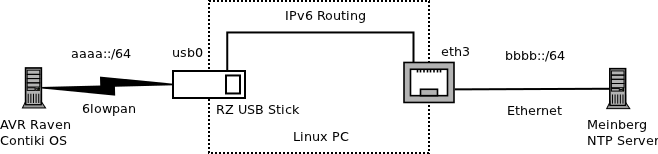
\includegraphics[width=13cm,keepaspectratio]{fig/radvd-routing.png}
	\caption{Contiki NTP Client communicating with the Meinberg NTP server}
	\label{fig:measurements-routing}
\end{figure}
Figure~\ref{fig:measurements-routing} shows the network topology used for the measurements.
The Meinberg~M600 NTP stratum 1 server synchronised using the GPS
was used as the reference clock for all of the presented measurements.
The NTP client was running on the AVR Raven platform in a room at 23~\textcelsius.

\section{Clock interrupt frequency}
For measuring clock interrupt frequency the bit 7 of Port D
and ground pin was connected to UNI-T~2025CEL digital oscilloscope.
At the beginning of the interrupt service routine a~logic 1 is written,
what causes a high level of voltage.
At the end of the interrupt service routine a~logic 0 is written,
what causes a low level of voltage.

When there is no clock adjustment, the value in output compare register is 31 by default.
The clock interrupt frequency
is supposed to be equal to a~value of the {\it{CLOCK\_SECOND}} macro, which is 128 by default on AVR~Raven.
The~figure~\ref{fig:app-osc-no-adjust} shows the output from oscilloscope
for this case.
$$\frac{\frac{f_{asy}}{prescaler}}{counts} = \frac{\frac{32768}{8}}{32} = 128$$

Figure~\ref{fig:app-osc-speed-up} shows the~output from oscilloscope
when slowing down the clock.
The~clock interrupt frequency
is supposed to be equal to $124.\overline{12}$~Hz.
$$\frac{\frac{f_{asy}}{prescaler}}{counts + 1} = \frac{\frac{32768}{8}}{32+1} = 124.\overline{12}$$

Figure~\ref{fig:app-osc-slow-down} shows the output from oscilloscope
when speeding up the clock.
The~clock interrupt frequency
is supposed to be approximately equal to 132.129~Hz.
$$\frac{\frac{f_{asy}}{prescaler}}{counts - 1} = \frac{\frac{32768}{8}}{32-1} \doteq 132.129$$

The~measured values are not exactly equal to those expected.
This is mostly due to influence of the clock source
(32~768~Hz quartz crystal oscillator) by a room temperature,
but it could also be air pressure or magnetic fields, etc.

\section{Clock offset}
\begin{figure}[H]
  \centering
  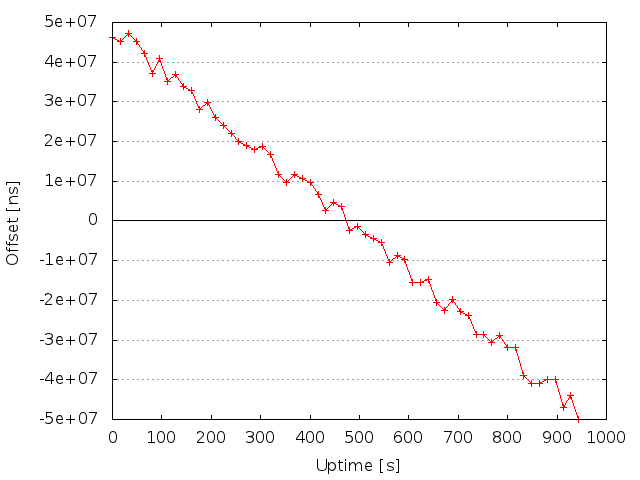
\includegraphics[width=11cm,keepaspectratio]{fig/no-ntp.png}
  \caption{Local clock offset without NTP client}
  \label{fig:measurements-no-ntp}
\end{figure}
Figure~\ref{fig:measurements-no-ntp} shows the local clock offset
in case no NTP client runs on the device.
The time is set with the initial offset of about 45 milliseconds.
However, the clock progresses faster due to frequency errors.
This compensates the initial clock offset at first,
but then it causes the offset increase.
The clock is running faster with approximately 100~PPM
(9 seconds a day) in this case and
the frequency jitter can be also observed.
The offset increase is therefore not exactly linear.

Figure~\ref{fig:measurements-ntp-serial} shows the local clock offset
acquired from the serial output when Contiki NTP Client runs on the device.
When the developed NTP client receives response from the server,
it calculates the local clock offset and prints this value to the serial output.
The NTP poll interval was set to 16 seconds, that means, the local clock offset
is calculated and eventually corrected every 16 seconds.
\begin{figure}[H]
  \centering
  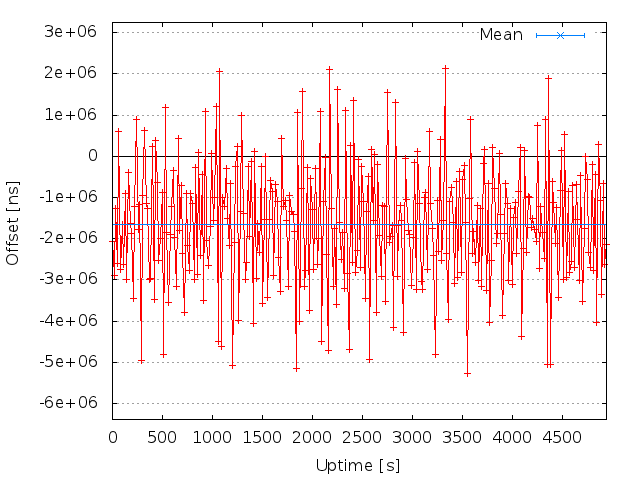
\includegraphics[width=11cm,keepaspectratio]{fig/poll-16s.png}
  \caption{Local clock offset with adjustments and NTP poll interval 16s}
  \label{fig:measurements-ntp-serial}
\end{figure}
The blue line shows the mean local clock offset value,
that should be equal to zero in a perfect case.
This is however not the case, because of oscillator frequency error
shown in figure~\ref{fig:measurements-no-ntp}.
More figures showing the local clock offset measurement
can be found in appendix~\ref{app:offset}.

\section{Clock phase}
The GPS based clock Meinberg~GPS~167 and digital oscilloscope UNI-T~2025CEL
was used for measuring the clock phase difference.
Meinberg~GPS clock rises an impulse when each second is accounted.
Contiki on AVR~Raven was configured to write a logic~1
to~bit~7 of~Port~D when each second is accounted,
and to write a logic~0 to~the same bit after~25 clock ticks.

When NTP client uses the {\it{clock\_adjust\_time}} call,
the local clock offset as well as the phase is being adjusted.
Figure~\ref{fig:measurements-osc-adjusting-phase} shows the phase while adjusting the clock.
The yellow line is the output signal from Meinberg~GPS clock
and the blue line is the output signal from AVR~Raven.
\begin{figure}[H]
  \centering
  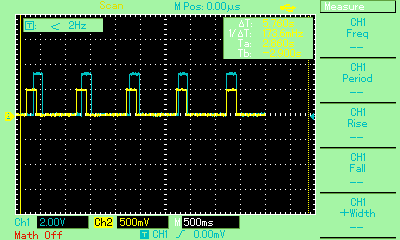
\includegraphics[width=11cm,keepaspectratio]{fig/osc-adjusting-phase.png}
  \caption{Second impulses when the clock is being adjusted}
  \label{fig:measurements-osc-adjusting-phase}
\end{figure}
Figures showing the clock out of phase and the clock in phase with
the reference clock can be found in appendix~\ref{app:phase}.
